\documentclass[conference]{IEEEtran}
\usepackage[a4paper]{geometry}
\usepackage{times,graphicx,amsmath,booktabs,cite,url}
\usepackage[ruled,linesnumbered]{algorithm2e}
\usepackage{array}

\begin{document}

\title{A Leakage-Free No-Code Workflow for Benchmarking Quantum Neural Networks on Small Tabular Data}

\author{\IEEEauthorblockN{Agrima Agarwal (230639), Aaradhya Gupta (230644),\\ Maheshwar Dwivedy, Kiran Khatter}
\IEEEauthorblockA{Group 01, School of Engineering \& Technology\\
BML Munjal University}}

\maketitle

\begin{abstract}
Quantum neural networks (QNNs) are often tested against weak or badly prepared classical baselines, and the people who want to test them usually need quantum programming skills they do not have. We built QNN Studio, a no-code workspace that takes a small table, cleans it, splits it, trains a simulated variational quantum classifier and four classical models, and reports the outcome with an honest confidence statement. The main design rule is that anything learned from data (gap filling, outlier limits, scaling, PCA) is fitted on the training rows only. Results come from several random splits, and the verdict ``ahead'', ``comparable'' or ``behind'' is read from a paired 95\% interval rather than from a single run. On five public datasets, a four-qubit QNN with 29 trainable parameters reached $93.8\pm1.3\%$ accuracy on breast-cancer diagnosis against $94.7\pm1.4\%$ for logistic regression, and was statistically behind the best classical model on only one of the five datasets. Ablations showed that circuit choice matters far more than depth: a basic entangling circuit lost 17.6 accuracy points, and a data-cleaning choice such as adding missing-value flags cost about five points. We did not observe any quantum advantage, and we explain why our setup cannot show one. The contribution is a reproducible, leakage-safe way to ask the question, together with a teaching mode that lets students repeat it.
\end{abstract}

\begin{IEEEkeywords}
benchmarking, data leakage, hybrid quantum-classical models, no-code tools, quantum neural networks, variational circuits
\end{IEEEkeywords}

\noindent\textbf{Overleaf Project Link:} \url{https://www.overleaf.com/project/6afdc87274f49166a796925a}

\section{Introduction}
Quantum machine learning (QML) has become a popular answer to the question of what quantum computers could be useful for. The idea is simple to state: encode data into the state of a few qubits, let a parameterised circuit transform it, measure, and train the circuit angles the same way we train the weights of a neural network~\cite{schuld2020circuit}. Today's machines are small and noisy, the regime Preskill called noisy intermediate-scale quantum (NISQ) computing~\cite{preskill2018nisq}, so most published QNN studies run on simulators with a handful of qubits and datasets that fit in a few hundred rows. Variational algorithms are the main candidate for useful work on such hardware~\cite{cerezo2021variational}, and early experiments suggested that quantum feature maps could separate data that is hard for classical kernels~\cite{havlicek2019supervised}.

That optimism has a quieter counterpart. Bowles, Ahmed and Schuld compared a dozen popular QML models against classical baselines and found that, once the classical models were set up properly, the quantum ones rarely came out ahead~\cite{bowles2024better}. Schuld and Killoran go further and ask whether beating classical accuracy should be the goal at all~\cite{schuld2022advantage}. K\"olle et al.\ take hybrid architectures apart to ask how much of the performance comes from the quantum circuit and how much from the classical layers around it~\cite{kolle2023disentangling}. In applied areas the same pattern appears. Medical benchmarks that pit quantum against classical models on cancer data exist~\cite{leither2026oncology}, and reviews of medical imaging describe a field with many promising small demonstrations and few controlled comparisons~\cite{shahriyar2025medical}. Breast cancer alone accounts for roughly 2.4 million new cases and about 694,000 deaths a year worldwide, according to the World Health Organization (WHO)~\cite{who2024breast}, which is part of why so many QML demonstrations choose this domain.

The problem we noticed, when we first tried to reproduce some of these experiments, is mundane. Each study builds its own data pipeline. Some scale the whole table before splitting, which quietly lets test information leak into training~\cite{kaufman2012leakage}. Some report one run on one split. Most need the reader to be comfortable with circuit libraries before they can change a single setting. A student or a domain scientist who simply wants to know whether a quantum model is any good on their own table has no safe way to find out.

\textbf{Gap.} We found tools that make quantum circuits easier to build, and papers that benchmark quantum models carefully, but we did not find an open workspace that combines the two and also forces the data-handling rules that make a benchmark believable: split first, fit on training rows only, repeat over seeds, compare with several classical baselines, and state a verdict from an interval rather than a point estimate.

This paper asks three research questions.
\begin{itemize}
  \item \textbf{RQ1.} On small public tabular datasets, how does a four-qubit hybrid QNN compare with standard classical baselines when every preparation step is leakage-free and every number is a mean over several splits?
  \item \textbf{RQ2.} Which circuit design choices (ansatz, data encoding, depth) change QNN accuracy the most?
  \item \textbf{RQ3.} How much do ordinary data-cleaning decisions move the result on a messy, realistic table?
\end{itemize}

Our contributions are the following.
\begin{itemize}
  \item QNN Studio, an open-source, no-code workspace with a seven-step research workflow (data, clean, prepare, model, train and compare, experiments, report) and a separate Learning Lab for teaching.
  \item A leakage-free preparation design in which structural cleaning is label-free and everything learned from data is fitted on training rows only, with the held-out rows transformed using training values.
  \item A verdict rule based on a paired 95\% confidence interval over matched random splits, which avoids declaring an advantage from a lucky run.
  \item A reproducible benchmark on five datasets plus circuit and cleaning ablations, with the scripts, data and code in a public repository.
\end{itemize}

The rest of the paper is organised as follows: Section~II reviews related work, Section~III formalises the problem, Section~IV describes the method, Section~V gives the experimental setup, Section~VI reports results, Section~VII discusses them, and Section~VIII concludes.

\section{Related Work}
We group the literature into four themes: what quantum models can and cannot express, how fairly they have been benchmarked, how QML has been applied to health and sports data, and how software tools support all of it.

\subsection{Quantum models as learning machines}
The circuit-centric classifier of Schuld et al.\ established the pattern we follow: encode a data point into qubits, apply a layered circuit with trainable rotations, and read out an expectation value~\cite{schuld2020circuit}. A later analysis showed that the data-encoding step decides which functions such a model can represent, so the choice of encoding is not cosmetic~\cite{schuld2021encoding}. In plain terms, a circuit that only ever sees one rotation per feature can produce only a limited family of smooth curves of that feature, however clever its trainable part is. That is one reason we compare encodings directly in our ablation instead of assuming angle encoding is good enough. Havl\'i\v{c}ek et al.\ proposed quantum-enhanced feature spaces and ran them on superconducting hardware~\cite{havlicek2019supervised}, and Cerezo et al.\ surveyed variational algorithms as a whole and their limits~\cite{cerezo2021variational}. The most cited obstacle for deeper circuits is the barren plateau, where gradients vanish exponentially with the number of qubits~\cite{mcclean2018barren}. We stay at four to eight qubits, where this problem is not the limiting factor, but we mention it because it bounds how far our conclusions can be extended. Fixing this problem is an active research topic, and nothing in our design claims to avoid it at larger sizes.

\subsection{Benchmarking quantum against classical}
Bowles et al.\ is the closest study to ours in spirit. They ran a large set of QML models, tuned the classical baselines properly, and found that the classical models generally won; they also found that removing the entangling gates from a quantum model often did not hurt it~\cite{bowles2024better}. K\"olle et al.\ separated the contribution of the quantum circuit from that of the classical layers in hybrid networks~\cite{kolle2023disentangling}. Schuld and Killoran argued that the field should look for structure that quantum models exploit instead of chasing accuracy tables~\cite{schuld2022advantage}. Statistical practice for comparing classifiers over several datasets has a longer history in classical machine learning~\cite{demsar2006statistical}, and we borrow its caution about reading too much into small differences. A related lesson from that literature is that a mean difference of one or two points over a handful of splits is easily produced by chance, which is why we report intervals alongside every comparison.

\subsection{Applications in health and sport}
Leither et al.\ benchmarked quantum and classical models on oncological data~\cite{leither2026oncology}, and Shahriyar and Tanbhir reviewed QML for medical image classification~\cite{shahriyar2025medical}. In sport, Baughman et al.\ studied which input features matter for QML models using fantasy-football data~\cite{baughman2022feature}. Classical machine learning for cricket is better developed: Shenoy et al.\ predicted Twenty20 match outcomes~\cite{shenoy2022t20}, and Mittal et al.\ studied player performance and match-result prediction~\cite{mittal2021player}. Taken together, these papers show that tabular health and sports data are realistic targets for quantum experiments, and that the classical side of the comparison is usually mature and strong, even though the sports studies do not use QNNs in the way we do.

\subsection{Tools and libraries}
PennyLane makes circuits differentiable and connects them to deep-learning frameworks~\cite{bergholm2018pennylane}. We use it with PyTorch~\cite{paszke2019pytorch}, and with scikit-learn for classical baselines and preprocessing~\cite{pedregosa2011sklearn}. These libraries are powerful but code-first. None of them enforces a particular data-handling discipline, which is exactly the thing that lets two people running ``the same'' experiment get different answers. Our contribution sits on top of them: we do not introduce a new quantum model, we package a disciplined way of using existing ones and make it accessible to people who cannot write the code.

\begin{table*}[!t]
\caption{Comparison of closely related work. ``Ours'' is the contribution of this paper.}
\label{tab:related}
\centering\footnotesize
\begin{tabular}{p{0.13\linewidth}p{0.19\linewidth}p{0.21\linewidth}p{0.32\linewidth}}
\toprule
Work & Problem & Method & Relevance and limit for our goal\\
\midrule
Schuld et al.~\cite{schuld2020circuit} & Quantum classifier design & Layered circuit, trainable rotations & Template for our circuit; no data-handling workflow\\
Havl\'i\v{c}ek et al.~\cite{havlicek2019supervised} & Quantum feature spaces & Feature map plus kernel/variational classifier on hardware & Motivates encodings; small synthetic data, no systematic baseline comparison\\
Bowles et al.~\cite{bowles2024better} & Fair benchmarking & Many QML models vs.\ tuned classical & Defines the standard we aim for; code-first, not a tool\\
K\"olle et al.~\cite{kolle2023disentangling} & Quantum vs.\ classical share in hybrids & Controlled architecture comparison & Separates quantum from classical contribution; no preparation workflow\\
Leither et al.~\cite{leither2026oncology} & Cancer data benchmarking & Quantum and classical models on oncology data & Same domain as one of our datasets; not interactive\\
Shahriyar and Tanbhir~\cite{shahriyar2025medical} & Medical image QML & Literature review & Shows need for controlled comparisons; review only\\
Baughman et al.~\cite{baughman2022feature} & Feature importance in QML & QML models on fantasy-football data & Sports use of QML; features, not a workflow\\
Shenoy et al.~\cite{shenoy2022t20} & T20 cricket outcome & Classical machine learning & Shows how strong classical sports models are; no quantum model\\
Ours & Leakage-free, repeatable QNN benchmarking for non-experts & No-code workspace, paired intervals, ablations & Combines tool, discipline and teaching mode; simulator and small data only\\
\bottomrule
\end{tabular}
\end{table*}

Table~\ref{tab:related} summarises the comparison. Reading across the rows, the pattern is clear. Papers that are careful about benchmarking are not tools that a newcomer can run, and tools that a newcomer can run do not enforce careful benchmarking. That is the gap this work fills, and it is also why we treat the paper's contribution as a workflow and an evaluation discipline rather than as a new quantum model.

\section{Background and Problem Formulation}
\subsection{Concepts and notation}
A qubit is the quantum counterpart of a bit. Its state can be rotated by an angle, and measuring it returns an average value between $-1$ and $+1$. A variational circuit is a short list of such rotations and two-qubit entangling gates, with some of the angles left free to be learned. A hybrid QNN places classical steps before and after the circuit. Training adjusts the free angles and the classical weights to reduce a loss on training rows, and we then judge the model on rows it has never seen.

\begin{table}[!t]
\caption{Notation used in this paper.}
\label{tab:notation}
\centering\footnotesize
\begin{tabular}{cp{0.68\linewidth}}
\toprule
Symbol & Meaning\\
\midrule
$q$ & number of qubits (also the number of model inputs)\\
$L$ & number of variational layers\\
$\mathbf{x}\in[0,\pi]^q$ & prepared feature vector of one row\\
$\boldsymbol{\theta}$ & trainable circuit angles\\
$\mathbf{w},b$ & weights and bias of the linear output head\\
$\langle Z_i\rangle$ & measured average of qubit $i$, in $[-1,1]$\\
$\mathcal{D}_\mathrm{tr},\mathcal{D}_\mathrm{ho}$ & training and held-out rows\\
$s$ & random seed, indexing one split and one initialisation\\
$S$ & number of seeds (runs)\\
$a_s$ & held-out accuracy (or $R^2$) of a model on run $s$\\
$d_s$ & paired difference between two models on run $s$\\
\bottomrule
\end{tabular}
\end{table}

Table~\ref{tab:notation} lists the symbols. Everywhere below, ``held-out'' means rows that were set aside before any preparation was fitted, and ``accuracy'' is the share of held-out rows classified correctly.

\subsection{Problem statement}
\textbf{Input.} A table with $n$ rows, $m$ feature columns of mixed type (numbers, categories, text, gaps) and one target column. The task is either classification or regression, detected from the target.

\textbf{Output.} For a quantum model and a set of classical baselines: held-out scores aggregated over $S$ seeds as mean and standard deviation, a paired 95\% interval of the quantum model minus each baseline, and a verdict in plain language, together with an audit trail of every cleaning step and a report that lets someone else repeat the study.

\textbf{Assumptions.} The table is small enough for exhaustive repetition (hundreds to a few thousand rows). The circuit is simulated exactly on a classical computer, with no shot noise or hardware noise. Rows are independent and identically distributed.

\textbf{Constraints.} No statistic computed from held-out rows may influence any step before evaluation. The number of qubits $q$ is small (we use 4 by default, up to 8). Run time on a laptop should be a few minutes per dataset.

\textbf{Out of scope.} Quantum hardware execution, noise mitigation, quantum kernels, image and time-series pipelines (an image demo exists in the repository but is not evaluated here), and any claim about asymptotic quantum advantage.

\section{Proposed Methodology}
\subsection{Architecture}
Fig.~\ref{fig:arch} shows the model. A prepared row enters an encoding layer that turns each of the $q$ numbers into a rotation on one qubit. A stack of $L$ variational layers follows, each with trainable single-qubit rotations and a ring of controlled-NOT gates that entangles neighbouring qubits. We then read out $\langle Z_i\rangle$ for every qubit and pass the $q$ readings to a linear head that produces class scores (classification) or a single value (regression). The circuit is a PennyLane QNode wrapped as a PyTorch layer, so one optimiser updates the circuit angles and the head together~\cite{bergholm2018pennylane,paszke2019pytorch}. We also offer three ansatz families (basic entangler, strongly entangling and hardware-efficient) and three encodings (angle, amplitude and IQP) so that the same data can be run through different designs. The interface shows the circuit diagram before training and counts the free angles, because we found that students who could see the circuit asked better questions about what was being learned.

\begin{figure*}[!t]
\centering
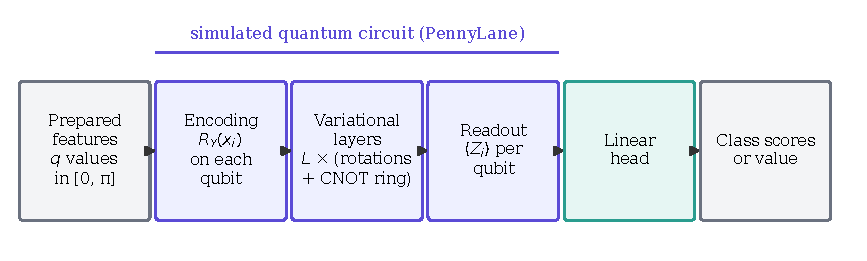
\includegraphics[width=0.85\textwidth]{figures/architecture.pdf}
\caption{Architecture of the hybrid model. The shaded middle stage runs on the simulated quantum circuit; the classical linear head converts the $q$ measured values into class scores or a regression value.}
\label{fig:arch}
\end{figure*}

With angle encoding, row $\mathbf{x}$ prepares the state
\begin{equation}
  |\psi(\mathbf{x})\rangle = \bigotimes_{i=1}^{q} R_Y(x_i)\,|0\rangle ,
  \label{eq:encode}
\end{equation}
where $R_Y(x_i)$ rotates qubit $i$ by the angle $x_i$. The variational block applies $U(\boldsymbol{\theta})=\prod_{l=1}^{L}\big(E\,\bigotimes_{i}R(\boldsymbol{\theta}_{l,i})\big)$, where $R(\cdot)$ is a general single-qubit rotation and $E$ is the ring of entangling gates. The readout is
\begin{equation}
  z_i(\mathbf{x};\boldsymbol{\theta}) = \langle\psi(\mathbf{x})|\,U^\dagger(\boldsymbol{\theta})\,Z_i\,U(\boldsymbol{\theta})\,|\psi(\mathbf{x})\rangle ,
  \label{eq:readout}
\end{equation}
and the model output is
\begin{equation}
  \hat{\mathbf{y}} = \mathbf{W}\mathbf{z} + \mathbf{b}, \qquad \mathbf{z}=(z_1,\dots,z_q)^\top .
  \label{eq:head}
\end{equation}
Here $\mathbf{W}$ and $\mathbf{b}$ are the head weights and biases. For $q=4$ and $L=2$ with the strongly entangling ansatz there are $24$ circuit angles and, with two classes, a head of $4\times 1+1$ parameters, giving the 29 trainable parameters reported later. The loss for classification is the cross-entropy and for regression the mean squared error on a standardised target, so that
\begin{equation}
  \mathcal{L} = \frac{1}{|\mathcal{B}|}\sum_{(\mathbf{x},y)\in\mathcal{B}} \ell\big(\hat{\mathbf{y}}(\mathbf{x}),y\big),
  \label{eq:loss}
\end{equation}
over a mini-batch $\mathcal{B}$, minimised with Adam~\cite{kingma2015adam}. Standardising the regression target does not change $R^2$ but keeps the bounded readouts from having to reproduce large raw values. We chose angle encoding as the default because it uses exactly $q$ gates for $q$ features, keeping circuits shallow; amplitude and instantaneous-quantum-polynomial (IQP) encodings are options for comparison~\cite{schuld2021encoding}. The price is that angle encoding is periodic: two raw values that differ by $2\pi$ would look identical, which is another reason we rescale into $[0,\pi]$ and clip held-out values so that each feature uses a half-period only once.

\subsection{Workflow}
Fig.~\ref{fig:workflow} gives the order of operations. The important decision is where the split sits. Structural cleaning uses no information about the target or about other rows' values: tidying text, converting numbers stored as text, removing duplicate rows, constant columns and identifier-like columns, and dropping rows or columns that are almost entirely empty. These steps are label-free and are safe to run before the split. Everything that learns a number from data runs after the split and is fitted on $\mathcal{D}_\mathrm{tr}$ only: gap filling with a training median, outlier limits set by a training interquartile range (IQR) rule, scaling, and either principal component analysis (PCA) or univariate feature selection down to $q$ columns. The held-out rows are then transformed using the numbers fitted on training rows, and finally clipped into the legal range so that an unusual held-out value cannot produce an angle outside $[0,\pi]$. We record every structural change with the number of rows and columns before and after, so the audit trail can be read by someone who did not run the study. The tool also computes a data-quality score between 0 and 100 from transparent deductions (for example for missing values, duplicates and identifier-like columns); the score guides the user but plays no part in the evaluation.

\begin{figure*}[!t]
\centering
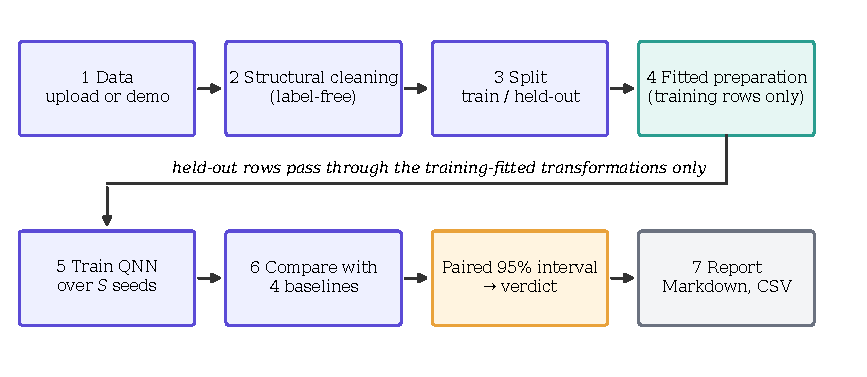
\includegraphics[width=0.85\textwidth]{figures/workflow.pdf}
\caption{Seven-step research workflow. Steps 3 and 4 enforce the leakage rule: the held-out rows pass through the transformations fitted on training rows and never contribute to them. The verdict uses a paired 95\% interval over seeds.}
\label{fig:workflow}
\end{figure*}

\begin{algorithm}[!t]
\caption{Leakage-free comparison study}
\label{alg:study}
\KwIn{Table $T$, configuration $C$ (qubits $q$, encoding, ansatz, layers $L$), number of seeds $S$}
\KwOut{Mean and standard deviation per model, paired intervals, verdict}
$T' \leftarrow$ structuralClean$(T)$ \tcp*{label-free}
\For{$s = 0,\dots,S-1$}{
  $(\mathcal{D}_\mathrm{tr},\mathcal{D}_\mathrm{ho}) \leftarrow$ split$(T', \text{seed}=s)$\;
  fit gap filler, outlier limits, scaler and PCA on $\mathcal{D}_\mathrm{tr}$ only\;
  transform $\mathcal{D}_\mathrm{tr}$ and $\mathcal{D}_\mathrm{ho}$ with the fitted objects; rescale to $[0,\pi]$ and clip\;
  train QNN on $\mathcal{D}_\mathrm{tr}$ with seed $s$; record $a_s^{\mathrm{QNN}}$ on $\mathcal{D}_\mathrm{ho}$\;
  \ForEach{baseline $B$}{
    train $B$ on the same $\mathcal{D}_\mathrm{tr}$; record $a_s^{B}$ on $\mathcal{D}_\mathrm{ho}$\;
  }
}
\ForEach{baseline $B$}{
  $d_s \leftarrow a_s^{\mathrm{QNN}}-a_s^{B}$; compute $\bar d \pm t_{0.975,S-1}\,\sigma_d/\sqrt{S}$\;
}
verdict $\leftarrow$ ``ahead'' if the interval is above 0, ``behind'' if below 0, else ``comparable''\;
\end{algorithm}

Algorithm~\ref{alg:study} spells the study out step by step. The choice to run the baselines on the very same prepared split as the QNN is deliberate. If the classical models saw richer features than the QNN, any gap would reflect preparation, not model class. Our baselines therefore all receive the same $q$ reduced columns. Splits are stratified by class for classification, and the same seed controls the split, the network initialisation and the mini-batch order, so a run can be repeated exactly. We acknowledge that this handicaps classical models relative to how they are normally used, and we report that in the discussion.

\subsection{Statistical verdict}
For each baseline $B$ and seed $s$ we compute $d_s=a_s^{\mathrm{QNN}}-a_s^{B}$. Because both models share a split, the pairing removes split-to-split variation that would otherwise swamp small differences. The interval is
\begin{equation}
  \bar d \pm t_{0.975,\,S-1}\;\frac{\sigma_d}{\sqrt{S}},
  \label{eq:paired}
\end{equation}
where $\bar d$ and $\sigma_d$ are the mean and sample standard deviation of the $d_s$. If the interval excludes zero we call the quantum model ahead or behind; otherwise comparable. For a single run the tool shows a Wilson interval on accuracy instead. Our earlier version of the tool used a cruder rule (``more than one standard deviation apart''), which overclaimed on small samples, so we replaced it. Using a $t$ interval with five runs is itself an approximation, since accuracies are bounded and not normally distributed, so we regard the verdict as a conservative guide rather than a formal test.

\subsection{Design reasons}
We keep $q$ small because the cost of exact simulation grows as $2^q$ and because the repeated-seed design multiplies it. We use Adam with a relatively large learning rate of 0.1 because we train for only 25 epochs and want the angles to move quickly; we did not tune this value. We scale features to $[0,\pi]$ rather than $[0,1]$ so that a rotation can cover half a turn and different rows end up in clearly different states. We insist on four classical baselines of different families, because beating a single weak baseline says little. Finally, we scale and reduce features before the circuit rather than inside it, because it keeps the number of qubits fixed regardless of the number of columns, and this is what lets a 100-column table run on four qubits at all.

\section{Experimental Setup}
\subsection{Data}
We use five public datasets, all small. Iris (150 rows, 4 features, 3 classes), Wine (178 rows, 13 features, 3 classes), and Breast Cancer Wisconsin Diagnostic (569 rows, 30 features, 2 classes)~\cite{wolberg1993wdbc} are classification tasks. The Diabetes progression data (442 rows, 10 features)~\cite{efron2004lars} is a regression task scored with $R^2$. To test scale we also use a synthetic table with 5,000 rows and 100 features. For the cleaning ablation we use a deliberately messy clinical table with 581 rows and 14 feature columns, containing gaps, numbers stored as text, duplicates and an identifier column; its target is benign versus malignant. In every study 25\% of rows are held out (for example 143 of 569 for breast cancer). The datasets are loaded from scikit-learn's bundled copies or generated by a seeded script, so no download is needed to reproduce the study.

\subsection{Tools and hardware}
Experiments ran on an Apple M5 laptop with 16 GB of memory, using CPU simulation only, with Python 3.14, PennyLane 0.45.1, PyTorch 2.14.0, scikit-learn 1.9.1, NumPy 2.5.3, pandas 2.3.3 and SciPy 1.18.1. The interface uses Streamlit and Plotly, and the repository includes a test suite of 95 tests that checks, among other things, that preparation does not use held-out rows.

\subsection{Baselines and metrics}
The classical baselines are logistic regression (ridge regression for the regression task), a support vector machine with a radial basis function kernel (SVM-RBF), a small multilayer perceptron (MLP) with hidden layers of 32 and 16 units, and a random forest of 200 trees. Accuracy is our classification metric because the classes are not extremely imbalanced and the number is easy to read; $R^2$ is the regression metric because it is independent of the target's units. We report standard deviations over seeds because they show how stable a model is, and training time because cost is part of any practical comparison. We deliberately do not report precision or recall in the main tables; the interface exposes a confusion matrix, but the datasets here are not extremely imbalanced and an extra metric would not change any verdict.

\begin{table}[!t]
\caption{Experimental parameters.}
\label{tab:params}
\centering\footnotesize
\begin{tabular}{lp{0.52\linewidth}}
\toprule
Parameter & Value\\
\midrule
Qubits $q$ & 4 (sweep: 2, 3, 4, 6, 8)\\
Encoding, ansatz, $L$ & angle, strongly entangling, 2\\
Reduction & PCA to $q$ components, rescaled to $[0,\pi]$\\
Optimiser, learning rate & Adam, 0.1 (0.05 for regression)\\
Epochs, batch size & 25 (30 for regression), 16 (32 for large table)\\
Held-out share & 25\%\\
Runs (seeds) per setting & $S=5$, seeds 0--4 (split and initialisation both change)\\
Confidence level & 95\% (paired $t$ interval)\\
Simulator & exact state vector, no noise, no shot sampling\\
\bottomrule
\end{tabular}
\end{table}

Table~\ref{tab:params} lists the settings. All seeds are fixed, so rerunning the script on the same library versions reproduces the numbers up to floating-point differences. The benchmark script is \texttt{scripts/run\_benchmark.py} and the ablations are in \texttt{scripts/run\_ablation.py}; both write JSON files from which every table and figure in this paper is generated.

\section{Results and Analysis}
\subsection{RQ1: quantum against classical baselines}
Table~\ref{tab:main} gives the main results and Fig.~\ref{fig:datasets} plots them. On Iris the QNN scored $94.2\pm6.0\%$, behind the MLP at $96.8\pm3.4\%$. On Wine it scored $93.3\pm2.7\%$ and SVM-RBF led at $97.3\pm1.9\%$. On breast cancer the QNN reached $93.8\pm1.3\%$, which is below the MLP ($95.2\pm2.0\%$) and logistic regression ($94.7\pm1.4\%$) but above the random forest ($92.9\pm1.8\%$). On the 5,000-row table it scored $96.3\pm0.9\%$, ahead of logistic regression ($95.1\pm0.6\%$) and behind SVM-RBF ($97.7\pm0.3\%$). On Diabetes the QNN reached $R^2=0.36\pm0.09$ against $0.42\pm0.03$ for ridge regression, and it beat the MLP and SVM.

\begin{table*}[!t]
\caption{Held-out score, mean $\pm$ standard deviation over 5 seeds (accuracy for the first four datasets, $R^2$ for Diabetes). Best value per column in bold. LR is logistic regression (ridge for Diabetes), RF is random forest.}
\label{tab:main}
\centering\footnotesize
\begin{tabular}{lccccc}
\toprule
Model & Iris & Wine & Breast cancer & 5,000$\times$100 & Diabetes\\
\midrule
QNN (29--39 params) & $.942\pm.060$ & $.933\pm.027$ & $.938\pm.013$ & $.963\pm.009$ & $.362\pm.093$\\
LR / ridge & $.963\pm.030$ & $.964\pm.012$ & $.947\pm.014$ & $.951\pm.006$ & $\mathbf{.418}\pm.032$\\
SVM-RBF & $.958\pm.040$ & $\mathbf{.973}\pm.019$ & $.945\pm.022$ & $\mathbf{.977}\pm.003$ & $.136\pm.020$\\
MLP (32, 16) & $\mathbf{.968}\pm.034$ & $.951\pm.033$ & $\mathbf{.952}\pm.020$ & $.976\pm.004$ & $.150\pm.197$\\
RF (200 trees) & $.958\pm.030$ & $.956\pm.022$ & $.929\pm.018$ & $.973\pm.005$ & $.319\pm.080$\\
\bottomrule
\end{tabular}
\end{table*}

\begin{figure*}[!t]
\centering
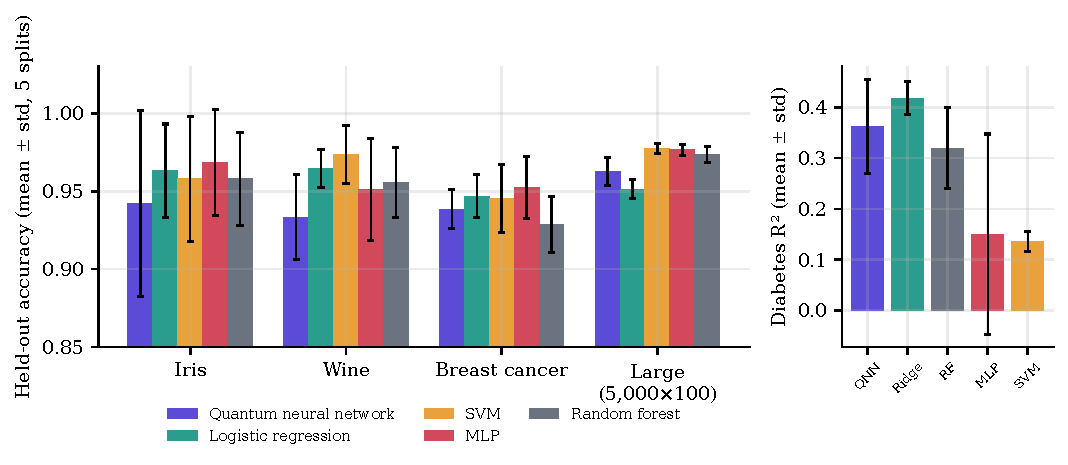
\includegraphics[width=0.85\textwidth]{figures/results_datasets.pdf}
\caption{Held-out results over five random splits. Left: accuracy on the four classification datasets. Right: $R^2$ on the Diabetes regression task. Error bars show one standard deviation across seeds.}
\label{fig:datasets}
\end{figure*}

These are raw differences; the paired intervals decide what they mean. On Iris, Wine and breast cancer, every interval against every baseline contains zero, so the verdict is ``comparable'', even though the QNN has the lowest mean on the first two. For example, on breast cancer the mean paired difference against logistic regression is $-0.8$ points with a half-width of $1.4$ points. On the large table the QNN is statistically behind SVM-RBF ($-1.5\pm1.1$ points) and the MLP ($-1.4\pm1.3$), comparable to the random forest and to logistic regression. On Diabetes it is comparable to ridge ($-5.6\pm10.0$ points of $R^2$) and clearly ahead of SVM-RBF ($+22.6\pm10.7$), whose weak score reflects a kernel poorly matched to this task more than any strength of the QNN. In summary, the QNN was never significantly ahead of the best classical model and was significantly behind it on one of five datasets. With only five seeds, intervals are wide and ``comparable'' should be read as ``not distinguished'', not as ``equal''. The broad pattern is that the QNN trails the best classical model by between one and four points, with the largest gap on Wine.

Efficiency tells a clearer story. The QNN needed 1.3 to 15.8 seconds to train a model on a laptop simulator, whereas logistic regression and SVM-RBF needed milliseconds and the MLP and forest a fraction of a second. The QNN is small (29 parameters, versus 705 for the MLP), which is its one notable advantage, but the comparison is not parameter-for-parameter fair either way.

\subsection{Sensitivity to qubits and training size}
Fig.~\ref{fig:sweeps} explores two settings on breast cancer. Increasing the number of qubits from 2 to 8 did not help the QNN: accuracy moved between $92.6\%$ and $94.0\%$ with no trend, while logistic regression improved from $93.4\%$ to $96.4\%$ as it received more PCA components. Run time rose from 2.0 s to 10.2 s. This is consistent with the view that the extra circuit capacity is not what limits the model here, and with the warnings about trainability of larger circuits~\cite{mcclean2018barren}. The right panel shows how both models learn from data. With 10\% of the training rows (42 samples) the QNN scored $89.5\%$ and logistic regression $91.7\%$; with all 426 rows the scores were $93.8\%$ and $94.7\%$. The curves run nearly parallel, so we found no sign that a quantum model uses small samples more efficiently, a hope sometimes raised for QML.

\begin{figure*}[!t]
\centering
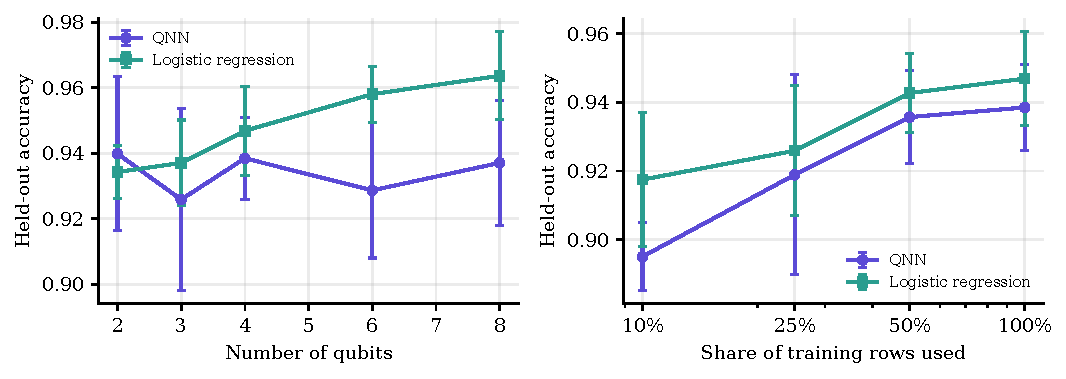
\includegraphics[width=0.85\textwidth]{figures/sweeps.pdf}
\caption{Breast-cancer sweeps (5 seeds, mean $\pm$ std). Left: accuracy against number of qubits. Right: accuracy against the share of training rows, on a log axis.}
\label{fig:sweeps}
\end{figure*}

\subsection{RQ2: circuit ablation}
Table~\ref{tab:ablation} and Fig.~\ref{fig:ablation} report seven circuit variants, each over the same five seeds on breast cancer, with the reference configuration first. The ansatz had the largest effect. Swapping the strongly entangling circuit for the basic entangler dropped accuracy from $93.8\%$ to $76.2\%$ (a 17.6 point loss) and made results unstable ($\pm6.5$). The basic entangler has only 8 trainable angles against 24, so some of this is lost capacity, but we did not test this explanation separately. A hardware-efficient circuit matched the reference ($93.7\pm1.7\%$). Encoding mattered next: amplitude encoding lost 3.2 points and IQP encoding 9.2. Depth mattered least. One layer lost 1.9 points, whereas four layers gained $0.3$ points, which is well inside the noise. A second layer is therefore worth having, but a fourth buys nothing here while doubling run time.

\begin{table}[!t]
\caption{Circuit ablation on breast cancer (accuracy, mean $\pm$ std over 5 seeds). $\Delta$ is the change from the reference in points.}
\label{tab:ablation}
\centering\footnotesize
\begin{tabular}{p{0.47\linewidth}cc}
\toprule
Variant & Accuracy & $\Delta$\\
\midrule
Reference (angle, strongly entangling, $L=2$) & $.938\pm.013$ & ---\\
Basic entangler ansatz & $.762\pm.065$ & $-17.6$\\
Hardware-efficient ansatz & $.937\pm.017$ & $-0.1$\\
Amplitude encoding & $.906\pm.028$ & $-3.2$\\
IQP encoding & $.846\pm.023$ & $-9.2$\\
1 layer & $.919\pm.013$ & $-1.9$\\
4 layers & $\mathbf{.941}\pm.019$ & $+0.3$\\
\midrule
Logistic regression (for scale) & $.947\pm.014$ & $+0.9$\\
\bottomrule
\end{tabular}
\end{table}

\begin{figure*}[!t]
\centering
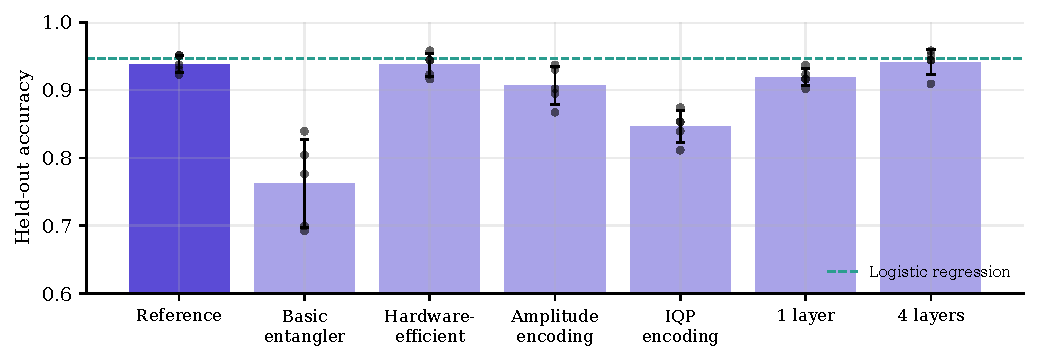
\includegraphics[width=0.85\textwidth]{figures/ablation_circuit.pdf}
\caption{Circuit ablation on breast cancer. Bars show the mean over five seeds with one standard deviation; dots are individual runs. The dashed line is logistic regression.}
\label{fig:ablation}
\end{figure*}

\subsection{RQ3: data-cleaning choices}
On the messy clinical table the cleaning choices moved results as much as some circuit choices did (Table~\ref{tab:clean}). With the recommended default (median gap filling, no outlier limit) the QNN scored $92.1\pm1.7\%$ and logistic regression $92.2\pm2.7\%$. Clipping extreme values at three IQRs gave the QNN $92.3\pm2.1\%$ and logistic regression $90.7\pm1.9\%$, the only configuration where the QNN scored higher on average, and by too small a margin and too few runs for us to call it a real advantage. Filling gaps with zero cost about 2.5 points, and adding missing-value flags cost about 4.7 points for the QNN and 4.0 for logistic regression. We suspect the flags change what PCA keeps among its four components, but we have not verified the cause. The point for practice is that the same data, with only the cleaning varied, can produce a spread larger than the quantum-versus-classical gap that the whole benchmark is trying to measure.

\begin{table}[!t]
\caption{Cleaning ablation on the messy clinical table (accuracy, mean $\pm$ std over 5 seeds).}
\label{tab:clean}
\centering\footnotesize
\begin{tabular}{p{0.40\linewidth}cc}
\toprule
Fitted-cleaning choice & QNN & LR\\
\midrule
Median fill, no outlier limit (default) & $.921\pm.017$ & $.922\pm.027$\\
Zero fill & $.896\pm.021$ & $.900\pm.012$\\
Median fill + missing flags & $.874\pm.019$ & $.882\pm.013$\\
Median fill + outlier clipping (3 IQR) & $\mathbf{.923}\pm.021$ & $.907\pm.019$\\
\bottomrule
\end{tabular}
\end{table}

\section{Discussion}
\subsection{What the results mean}
The picture across all experiments is consistent. A small simulated QNN is a respectable classifier on small tables, usually within a couple of points of the classical models, and almost never distinguishable from them with only five runs. That agrees with the careful benchmark of Bowles et al.~\cite{bowles2024better} and with the argument of Schuld and Killoran that accuracy alone is a poor target~\cite{schuld2022advantage}. Our ablations add a practical lesson in the same spirit as K\"olle et al.~\cite{kolle2023disentangling}: the surrounding choices (ansatz, encoding, preparation) move accuracy more than the amount of quantum depth does.

For a researcher, the practical meaning is that a QNN result without a leakage-safe pipeline, several seeds and baselines receiving the same inputs is difficult to interpret. For a student, the benefit is that all of this can be done by clicking through the workspace, and the Learning Lab explains each step in plain language. We have not measured the teaching benefit and say so below.

\subsection{Limitations and threats to validity}
\textbf{Internal validity.} Five seeds is few; intervals are wide, and a true difference of one or two points would be missed. We did not tune any model beyond defaults, including the QNN, so every comparison is between default configurations. Our classical baselines see only $q=4$ PCA components, which is unusually restrictive for them. That choice makes the comparison fair in inputs but probably understates how well classical models do on the full tables, which means the QNN's standing in a ``best-effort'' contest would be worse than reported here. The IQP and amplitude results depend on our implementations and on the small number of seeds.

\textbf{Construct validity.} Accuracy and $R^2$ on a single held-out quarter do not capture calibration, class imbalance effects, or clinical usefulness.

\textbf{External validity.} Our datasets are small, public and clean enough that classical models are near their ceiling, so there is little room for any model to show an advantage. The circuit is simulated without noise, so our results say nothing about hardware. The messy clinical table is a constructed example and the cleaning conclusions may not transfer.

\textbf{Conclusion validity.} We ran many comparisons without correction for multiple testing, and we draw conclusions from the pattern, not from any single interval.

\subsection{Ethics and responsible use}
Two of our datasets are medical. The tool is for learning and research, and it should not support clinical decisions, a position consistent with WHO guidance on the ethics and governance of artificial intelligence for health~\cite{who2021ethics}. The datasets are public and de-identified, and we did not collect any personal data. The workspace states on its first page that a ``comparable'' result is not evidence of quantum advantage.

\section{Conclusion and Future Work}
We set out to make quantum-versus-classical comparisons easy to run and hard to get wrong, and to use the resulting workspace to ask three questions.

\textbf{RQ1.} With leakage-free preparation and five seeds, the four-qubit QNN was comparable to the classical baselines in most comparisons and significantly behind the best of them on one of five datasets, for example $93.8\pm1.3\%$ against $94.7\pm1.4\%$ for logistic regression on breast cancer. \textbf{RQ2.} The choice of ansatz and encoding changed accuracy by up to 17.6 points, much more than going from one to four layers, which changed it by 1.9 points at most. \textbf{RQ3.} Cleaning choices moved accuracy by up to about five points on a messy table, which is as large as the quantum-classical differences we were trying to measure.

We did not find a quantum advantage, and our setup (small tables, a noiseless simulator, handicapped baselines) is not designed to find one. What we can offer is a reproducible method and tool whose verdicts are conservative.

Three directions follow. First, repeat the benchmark with more seeds and tuned classical baselines given the full feature set. Second, run the same pipeline on a small number of real quantum-hardware or noisy-simulator backends. Third, run a controlled classroom study to measure whether the Learning Lab improves understanding, which we have not yet done.

\section*{Declarations}
\textbf{Source code and data.} \url{https://github.com/aaradhya1205/qnn-platform}. All figures and tables are generated from the JSON outputs of the scripts in the repository.

\textbf{AI-use declaration.} An AI assistant (Claude, by Anthropic) was used heavily in this project. It helped write and debug the QNN Studio code, wrote the experiment and plotting scripts, suggested the experimental design, and produced the first draft of this report, including its text, tables and figures. The group chose the project topic, directed the work, ran the code on its own machine, reviewed the outputs and the draft, and takes responsibility for the content. All reported numbers were produced by the scripts in the repository, not typed from memory. The reference list was assembled with the assistant's help and should be read as checked by the group against the original sources.

\textbf{Contribution statement.} Both members contributed equally to all parts of the project.
\begin{itemize}
  \item Agrima Agarwal (230639): shared equally in designing the study, building and testing the platform, running the experiments, and writing and reviewing the report.
  \item Aaradhya Gupta (230644): shared equally in designing the study, building and testing the platform, running the experiments, and writing and reviewing the report.
\end{itemize}

\bibliographystyle{IEEEtran}
\bibliography{references}

\end{document}
